\documentclass[aspectratio=169]{beamer}
\usetheme{metropolis}

\usepackage{graphicx}
\usepackage{listings}
\usepackage{xcolor}

% --- TikZ (Flowcharts) ---
\usepackage{tikz}
\usetikzlibrary{shapes.geometric, arrows.meta, positioning}

% Define custom colors for listings
\definecolor{codegreen}{rgb}{0,0.6,0}
\definecolor{codegray}{rgb}{0.5,0.5,0.5}
\definecolor{codepurple}{rgb}{0.58,0,0.82}
\definecolor{backcolour}{rgb}{0.96,0.96,0.96}

\lstdefinestyle{mystyle}{
    backgroundcolor=\color{backcolour},
    commentstyle=\color{codegreen},
    keywordstyle=\color{blue},
    numberstyle=\tiny\color{codegray},
    stringstyle=\color{codepurple},
    basicstyle=\ttfamily\small,
    breakatwhitespace=false,
    breaklines=true,
    captionpos=b,
    numbers=left,
    numbersep=5pt,
    showspaces=false,
    showstringspaces=false,
    showtabs=false,
    tabsize=2
}

\lstset{style=mystyle}

% --- TikZ styles for flowcharts ---
\tikzstyle{startstop} = [ellipse, draw, minimum width=2.8cm, minimum height=0.9cm, align=center]
\tikzstyle{process}   = [rectangle, draw, minimum width=3.4cm, minimum height=0.9cm, align=center]
\tikzstyle{decision}  = [diamond, draw, aspect=2.2, inner sep=1pt, align=center]
\tikzstyle{arrow}     = [-{Stealth[length=2.2mm]}, thick]

\title{Python 3 - Grundlagen und Ökosystem}
\subtitle{Unit 1: Programmiergrundlagen, Flussdiagramme \& Python-Tooling}
\author{Hussam Alafandi}
\date{\today}

\begin{document}

\maketitle

% =========================================================
% Unit Overview
% =========================================================
\section{Unit 1: Überblick}

\begin{frame}{Ziele der Unit}
  \begin{itemize}
    \item Verstehen, was Programmierung ist (Problem $\rightarrow$ Algorithmus $\rightarrow$ Code).
    \item Kontrollfluss verstehen: Sequenz, Entscheidung, Wiederholung.
    \item Flussdiagramme (Flowcharts) als Planungswerkzeug nutzen.
    \item Verstehen, wie Python Code ausführt (Interpreter, Skripte, Notebooks).
    \item Entwicklungsumgebungen nutzen: Jupyter und VS Code.
    \item Virtuelle Umgebungen einsetzen (venv, conda).
    \item Pakete und Abhängigkeiten verwalten (pip, requirements.txt).
  \end{itemize}
\end{frame}

\begin{frame}{Agenda}
  \begin{enumerate}
    \item Programmieren als Problemlösen
    \item Kontrollfluss \& Flussdiagramme (TikZ)
    \item Brücke zu Python
    \item Python-Tooling: Interpreter, Skripte, Notebooks
    \item Setup: Umgebungen, Pakete, Praxis
    \item Aufgaben
  \end{enumerate}
\end{frame}

% =========================================================
% Part 1: Programming Fundamentals
% =========================================================
\section{Programmieren als Problemlösen}

\begin{frame}{Warum zuerst die Konzepte?}
  \begin{itemize}
    \item Programmierung ist Problemlösen, nicht Syntax.
    \item Logik ist universell: unabhängig von Python, Java, \dots
    \item Gute mentale Modelle reduzieren spätere Fehler.
    \item Wir planen erst, dann implementieren wir.
  \end{itemize}
\end{frame}

\begin{frame}{Was ist Programmierung?}
  \begin{itemize}
    \item Programmierung bedeutet, einem Computer klare Anweisungen zu geben.
    \item Computer sind deterministisch: gleiche Eingabe $\rightarrow$ gleiche Ausgabe.
    \item Ziel: Ein konkretes Problem zuverlässig lösen.
  \end{itemize}
\end{frame}

\begin{frame}{Von Problem zu Lösung}
  \textbf{Allgemeiner Ablauf:}
  \begin{enumerate}
    \item Problem verstehen
    \item Algorithmus entwerfen
    \item Implementieren (Code)
    \item Testen und verbessern
  \end{enumerate}
\end{frame}

\begin{frame}{Was ist ein Algorithmus?}
  \begin{itemize}
    \item Schritt-für-Schritt-Anleitung zur Lösung eines Problems.
    \item Eindeutig, nachvollziehbar und reproduzierbar.
    \item Unabhängig von Programmiersprachen.
  \end{itemize}
\end{frame}

% =========================================================
% Control Flow + Flowcharts
% =========================================================
\section{Kontrollfluss \& Flussdiagramme}

\begin{frame}{Kontrollfluss: Die drei Grundbausteine}
  \begin{itemize}
    \item \textbf{Sequenz:} Anweisungen nacheinander
    \item \textbf{Entscheidung:} Verzweigung anhand einer Bedingung
    \item \textbf{Wiederholung:} Schritte mehrfach ausführen
  \end{itemize}
\end{frame}

\begin{frame}{Flowcharts: Symbole}
  \begin{itemize}
    \item Oval: Start / Ende
    \item Rechteck: Aktion / Verarbeitung
    \item Raute: Entscheidung
    \item Pfeile: Kontrollfluss
  \end{itemize}
\end{frame}

% ---------------------------------------------------------
% TikZ Flowchart 1: Number classification
% ---------------------------------------------------------
\begin{frame}{Flowchart-Beispiel: Zahl klassifizieren}
  \centering
  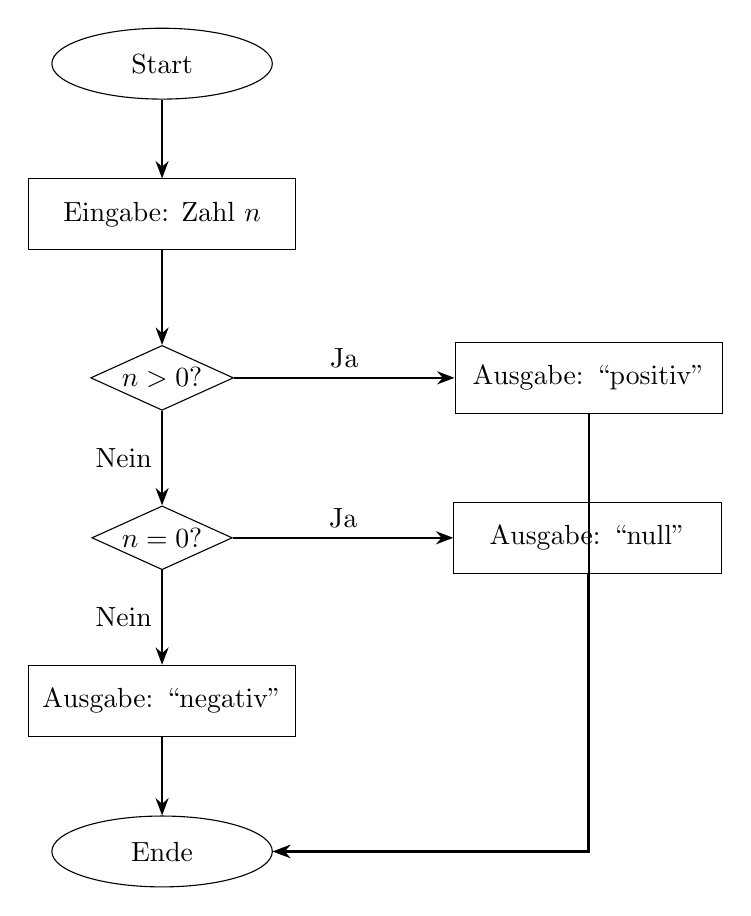
\begin{tikzpicture}[node distance=1.0cm]
    \node (start) [startstop] {Start};
    \node (input) [process, below=of start] {Eingabe: Zahl $n$};
    \node (d1) [decision, below=of input, yshift=-0.2cm] {$n > 0$?};
    \node (pos) [process, right=2.8cm of d1] {Ausgabe: ``positiv''};
    \node (d2) [decision, below=of d1, yshift=-0.2cm] {$n = 0$?};
    \node (zero) [process, right=2.8cm of d2] {Ausgabe: ``null''};
    \node (neg) [process, below=of d2, yshift=-0.2cm] {Ausgabe: ``negativ''};
    \node (stop) [startstop, below=of neg] {Ende};

    \draw [arrow] (start) -- (input);
    \draw [arrow] (input) -- (d1);

    \draw [arrow] (d1) -- node[above]{Ja} (pos);
    \draw [arrow] (pos) |- (stop);

    \draw [arrow] (d1) -- node[left]{Nein} (d2);

    \draw [arrow] (d2) -- node[above]{Ja} (zero);
    \draw [arrow] (zero) |- (stop);

    \draw [arrow] (d2) -- node[left]{Nein} (neg);
    \draw [arrow] (neg) -- (stop);
  \end{tikzpicture}
\end{frame}

\begin{frame}{Interpretation des Flowcharts}
  \begin{itemize}
    \item \textbf{Sequenz:} Start $\rightarrow$ Eingabe $\rightarrow$ Prüfung
    \item \textbf{Entscheidung:} Zwei Verzweigungen ($n>0$?, $n=0$?)
    \item \textbf{Determinismus:} Für jedes $n$ genau ein Pfad
    \item Das ist später direkt übersetzbar in \texttt{if/elif/else}.
  \end{itemize}
\end{frame}

% ---------------------------------------------------------
% TikZ Flowchart 2: Login with retry loop
% ---------------------------------------------------------
\begin{frame}{Flowchart-Übung: Login mit Wiederholung}
  \centering
  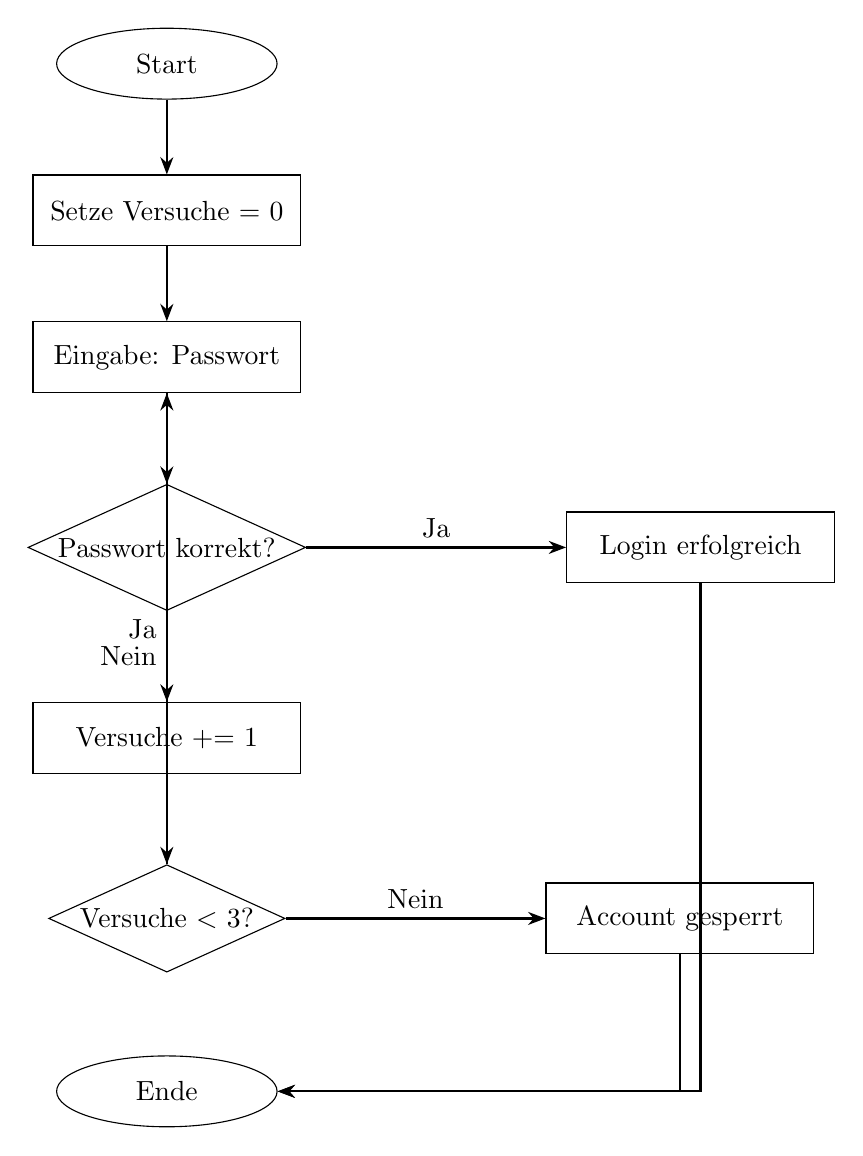
\begin{tikzpicture}[node distance=0.95cm]
    \node (start) [startstop] {Start};
    \node (set) [process, below=of start] {Setze Versuche = 0};
    \node (input) [process, below=of set] {Eingabe: Passwort};
    \node (check) [decision, below=of input, yshift=-0.2cm] {Passwort korrekt?};
    \node (ok) [process, right=3.3cm of check] {Login erfolgreich};
    \node (inc) [process, below=of check, yshift=-0.2cm] {Versuche += 1};
    \node (limit) [decision, below=of inc, yshift=-0.2cm] {Versuche $<$ 3?};
    \node (fail) [process, right=3.3cm of limit] {Account gesperrt};
    \node (stop) [startstop, below=of limit, yshift=-0.1cm] {Ende};

    \draw [arrow] (start) -- (set);
    \draw [arrow] (set) -- (input);
    \draw [arrow] (input) -- (check);

    \draw [arrow] (check) -- node[above]{Ja} (ok);
    \draw [arrow] (ok) |- (stop);

    \draw [arrow] (check) -- node[left]{Nein} (inc);
    \draw [arrow] (inc) -- (limit);

    \draw [arrow] (limit) -- node[above]{Nein} (fail);
    \draw [arrow] (fail) |- (stop);

    \draw [arrow] (limit) -- node[left]{Ja} (input);
  \end{tikzpicture}
\end{frame}


% =========================================================
% Bridge to Python
% =========================================================
\section{Brücke zu Python}

\begin{frame}{Von Flowchart zu Python}
  \begin{itemize}
    \item Flowchart beschreibt \textbf{Logik} und \textbf{Kontrollfluss}.
    \item Python bietet konkrete Sprachkonstrukte:
          \begin{itemize}
            \item Sequenz: Zeile für Zeile
            \item Entscheidung: \texttt{if/elif/else}
            \item Wiederholung: \texttt{for/while}
          \end{itemize}
    \item Nächster Schritt: Setup, damit wir diese Logik sauber implementieren können.
  \end{itemize}
\end{frame}

% =========================================================
% Part 2: Python Ecosystem & Tooling
% =========================================================
\section{Python: Interpreter, Skripte, Notebooks}

\begin{frame}{Wie führt Python Code aus?}
  \begin{itemize}
    \item Python ist eine interpretierte Sprache: Code wird durch den \textbf{Interpreter} ausgeführt.
    \item Quellcode-Dateien enden meist auf \texttt{.py}.
    \item Interaktiv vs. Datei-basiert:
          \begin{itemize}
            \item Interaktiv: Python REPL (Shell)
            \item Datei-basiert: Skripte (\texttt{python file.py})
          \end{itemize}
  \end{itemize}
\end{frame}

\begin{frame}{Skripte vs. Notebooks}
  \begin{itemize}
    \item \textbf{Skripte:}
          \begin{itemize}
            \item Gut für wiederholbare Abläufe und Softwareentwicklung
            \item Saubere Projektstruktur
            \item Einfach zu versionieren (Git)
          \end{itemize}
    \item \textbf{Notebooks:}
          \begin{itemize}
            \item Gut für Exploration, Lernen, Datenanalyse
            \item Mischung aus Code, Text, Output
            \item Achtung: ``Hidden State'' durch nicht-lineare Ausführung
          \end{itemize}
  \end{itemize}
\end{frame}

\section{Entwicklungsumgebungen}

\begin{frame}{Jupyter Notebook}
  \begin{itemize}
    \item Interaktive Umgebung für Code + Markdown + Visualisierungen.
    \item Ideal für Lernen, Exploration und Reports.
  \end{itemize}
\end{frame}

\begin{frame}{VS Code}
  \begin{itemize}
    \item Professioneller Editor für Projekte.
    \item Vorteile:
          \begin{itemize}
            \item Autocomplete \& Linting
            \item Debugging
            \item Integriertes Terminal
            \item Git-Integration
            \item Notebook-Support
          \end{itemize}
  \end{itemize}
\end{frame}

\section{Praxis: Installation \& Checks}

\begin{frame}[fragile]{Python Installation prüfen}
  \begin{itemize}
    \item Version prüfen:
          \begin{lstlisting}[language=bash]
python --version
python3 --version
\end{lstlisting}
    \item Wo liegt der Interpreter?
          \begin{lstlisting}[language=bash]
which python      # Mac/Linux
where python      # Windows
\end{lstlisting}
  \end{itemize}
\end{frame}

\begin{frame}[fragile]{Erste Python-Kommandos (REPL)}
  \begin{itemize}
    \item Python Shell starten:
          \begin{lstlisting}[language=bash]
python
\end{lstlisting}
    \item Erste Befehle:
          \begin{lstlisting}[language=Python]
print("Hallo Python!")
2 + 3 * 4
\end{lstlisting}
    \item Verlassen:
          \begin{lstlisting}[language=Python]
exit()
\end{lstlisting}
  \end{itemize}
\end{frame}

% =========================================================
% Environments
% =========================================================
\section{Virtuelle Umgebungen}

\begin{frame}{Warum virtuelle Umgebungen?}
  \begin{itemize}
    \item Vermeidung von Versionskonflikten zwischen Projekten.
    \item Reproduzierbarkeit (gleiche Pakete $\rightarrow$ gleiche Ergebnisse).
    \item Saubere Abhängigkeiten pro Projekt.
  \end{itemize}
\end{frame}

\begin{frame}[fragile]{Virtuelle Umgebung mit venv}
  \textbf{Schritte:}
  \begin{enumerate}
    \item Umgebung erstellen:
          \begin{lstlisting}[language=bash]
python -m venv .venv
\end{lstlisting}
    \item Aktivieren:
          \begin{lstlisting}[language=bash]
source .venv/bin/activate      # Mac/Linux
.venv\Scripts\activate         # Windows
\end{lstlisting}
    \item Deaktivieren:
          \begin{lstlisting}[language=bash]
deactivate
\end{lstlisting}
  \end{enumerate}
\end{frame}

\begin{frame}[fragile]{Virtuelle Umgebung mit Conda}
  \textbf{Schritte:}
  \begin{enumerate}
    \item Umgebung erstellen:
          \begin{lstlisting}[language=bash]
conda create --name py101 python=3.11
\end{lstlisting}
    \item Aktivieren:
          \begin{lstlisting}[language=bash]
conda activate py101
\end{lstlisting}
    \item Deaktivieren:
          \begin{lstlisting}[language=bash]
conda deactivate
\end{lstlisting}
  \end{enumerate}
\end{frame}

\begin{frame}{venv vs. Conda (Kurzvergleich)}
  \begin{itemize}
    \item \textbf{venv:} eingebaut, leichtgewichtig, gut für ``pure Python''.
    \item \textbf{Conda:} stark im wissenschaftlichen Umfeld, eigene Paketverwaltung.
  \end{itemize}
\end{frame}

% =========================================================
% Dependencies
% =========================================================
\section{Pakete \& Abhängigkeiten}

\begin{frame}{Standard Library vs. Third-Party}
  \begin{itemize}
    \item \textbf{Standard Library:} kommt mit Python (z.\,B. \texttt{math}, \texttt{csv}, \texttt{json}).
    \item \textbf{Third-Party:} installierbar via \texttt{pip}/\texttt{conda} (z.\,B. \texttt{numpy}, \texttt{pandas}).
    \item Ziel: reproduzierbares Setup über \texttt{requirements.txt}.
  \end{itemize}
\end{frame}

\begin{frame}[fragile]{Pakete installieren mit pip}
  \begin{itemize}
    \item Installation:
          \begin{lstlisting}[language=bash]
pip install numpy pandas
\end{lstlisting}
    \item Export:
          \begin{lstlisting}[language=bash]
pip freeze > requirements.txt
\end{lstlisting}
    \item Re-Install:
          \begin{lstlisting}[language=bash]
pip install -r requirements.txt
\end{lstlisting}
  \end{itemize}
\end{frame}

% =========================================================
% Script vs Notebook practice
% =========================================================
\section{Praxis: Skript vs. Notebook}

\begin{frame}[fragile]{Einfaches Skript: \texttt{hello.py}}
  \begin{lstlisting}[language=Python]
print("Hallo aus einem Skript!")
x = 2 + 3 * 4
print("Ergebnis:", x)
\end{lstlisting}
\end{frame}

\begin{frame}{Notebook: gleiche Logik, andere Arbeitsweise}
  \begin{itemize}
    \item Code in Zellen, Markdown für Dokumentation, Output direkt sichtbar.
    \item Achtung: Reihenfolge der Ausführung kann den Zustand beeinflussen.
    \item Empfehlung: Notebooks reproduzierbar halten (``Run All'').
  \end{itemize}
\end{frame}

% =========================================================
% Assignments
% =========================================================
\section{Aufgaben (Unit 1)}

\begin{frame}{Aufgabe 0: Flussdiagramm (ohne Code)}
  \begin{itemize}
    \item Entwerfe ein Flussdiagramm für:
          \begin{itemize}
            \item Anmeldung an einem System (max. 3 Versuche)
          \end{itemize}
  \end{itemize}
\end{frame}

\begin{frame}{Aufgabe 1: Setup \& Dokumentation}
  \begin{itemize}
    \item Python-Version prüfen und dokumentieren.
    \item Virtuelle Umgebung erstellen und aktivieren.
    \item \texttt{numpy} installieren.
    \item Schritte in \texttt{environment\_setup.md} dokumentieren.
  \end{itemize}
\end{frame}

\begin{frame}{Aufgabe 2: Skript vs. Notebook}
  \begin{itemize}
    \item Erstelle \texttt{hello.py} und \texttt{hello.ipynb} mit:
          \begin{itemize}
            \item Ausgabe einer Begrüßung
            \item Einer einfachen Berechnung
          \end{itemize}
    \item Führe beide aus und vergleiche den Ablauf.
  \end{itemize}
\end{frame}

\begin{frame}{Aufgabe 3: Kurzreflexion}
  \begin{itemize}
    \item Beantworte kurz:
          \begin{enumerate}
            \item Was macht der Python Interpreter?
            \item Wann ist ein Notebook sinnvoller als ein Skript?
            \item Warum sind virtuelle Umgebungen nützlich?
          \end{enumerate}
  \end{itemize}
\end{frame}

\begin{frame}[standout]
  \huge Fragen?
\end{frame}

\end{document}
